\documentclass[12pt]{report}

\usepackage[T1]{fontenc}
\usepackage[utf8]{inputenc}
\usepackage{graphicx}

\begin{document}
 
\title{\textbf{ Los arreglos y parametros de los Amplificadores Clase A\\
\includegraphics[scale=0.5]{upzmg.jpg}}}
\author{Enesto Alonso Partida López\\ Universidad Politecnica De La Zona Metropolitana De Guadalajara\\ Mecatronica 4 A\\ Septiembre-diciembre 2019}

\date{1 de octubre 2019 }
\maketitle

\newpage
{\huge \textbf{¿Qué es un Amplificador de tipo A?}\\}\\


{\large Amplificador clase A. Son aquellos amplificador cuyas etapas de potencia consumen corrientes altas y continuas de su fuente de alimentación, independientemente de si existe señal de audio o no.}\\
 

{\huge \textbf{¿Comó se clasifican los amplificadores?}\\}\\


{\large Se clasifican principalmente por la frecuencia con la que estos trabajan, asi se conocen las clase A, B, AB y C las cuales tiene difentes usos y aplicaciones, ademas,estos se dividen en amplificadores de potencia y tensión, en este caso solo nos centraremos en los Amplificadores de tipo A}\\
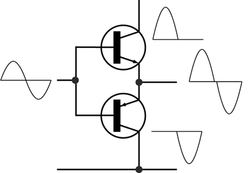
\includegraphics[scale=0.7]{../../../Downloads/descragas/amplicador.png}\\


{\huge \textbf{Amplificador de tensión y potencia}\\}\\


{\large Los aplificadores de tension son aquellos que suministran una mayor tension en su salida, cuando su tension de entrada es menor. Por otro lado tenemos los aplificadores de potencia los cuales al igual que los de tension, su tension es mayor en la salida que en la entrada, pero a demas, su corriente es mucho mayor en la salida que en la entrada. Por eso su nombre de amplificadores de potencia }\\
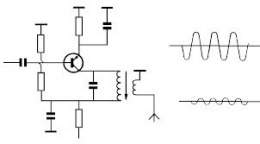
\includegraphics[scale=1]{../../../Downloads/descragas/AmplificadorclaseAtension.jpg} \\
{\huge \textbf{Funcionamiento de un amplificador de potencia clase A}\\}\\

{\large Un amplificador de potencia funciona en clase A cuando la tensión de polarización y la amplitud máxima de la señal de entrada poseen valores tales que hacen que la corriente de salida circule durante todo el período de la señal de entrada.  Y la diferncia que tiene con un amplificador de tipo B es que el amplificador clase B su corriente de salida circula durante un semiperíodo de la señal de entrada.\\ En los amplificadore snunca existira una corrinete de reja(base.}\\
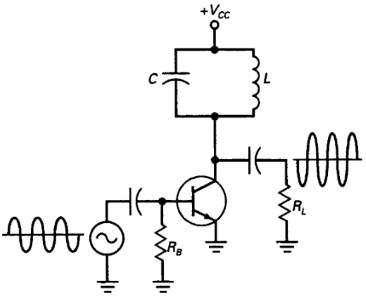
\includegraphics[scale=0.7]{../../../Downloads/descragas/amplificadores.png} 

{\huge \textbf{ventaja y desventaje de los amplificadores clase A}\\}\\


{\large La clase A se refiere a una etapa de salida con una corriente de polarización mayor que la máxima 
corriente de salida que dan, de tal forma que los transistores de salida siempre están consumiendo corriente. La gran ventaja de la clase A es que es casi lineal, y en consecuencia la distorsión es menor.\\ Y su gran desventaja de la clase A es que es poco eficiente, se requiere un amplificador de clase A muy grande para dar 50 W, y ese amplificador usa mucha corriente y se pone a muy alta temperatura.

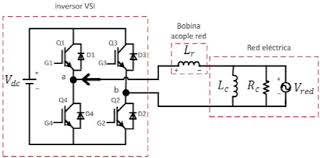
\includegraphics[scale=1]{../../../Downloads/descragas/descarga.jpg} 
\newpage
{\huge \textbf{Bibliografia:}\\}\\
@online{Electronica Unicrom,
author = {Luis González López},
title = {Amplificadores de Potencia: clasificación, clase A, B, AB, C},
year = {2016},
url = {https://unicrom.com/amplificadores-de-potencia-clasificacion/},
OPTsubtitle = {Amplificadores clase A},
OPTlanguage = {Español},
OPTversion = {1},
OPTdate = {21},
OPTmonth = {6},
OPTurldate = {https://unicrom.com/amplificadores-de-potencia-clasificacion/},
}


\end{document}